\documentclass{article}
\usepackage{../m}
\usepackage[pdftex]{graphicx}

\begin{document}
\noindent Paul Gustafson\\
\noindent Texas A\&M University - Math 641\\ 
\noindent Instructor - Fran Narcowich

\subsection*{HW 2}
\p{1 a} Show that if $\alpha$, $\beta$ are positive with $\alpha + \beta = 1$ then for all $u,v \ge 0$ we have
$$ u^\alpha v^\beta \le \alpha u + \beta v.$$
\begin{proof} If $u = v = 0$, then the inequality holds. Since the inequality is symmetric in $u$ and $v$, we may assume $v \neq 0$.
Hence we wish to show
$$(\frac u v)^\alpha \le \alpha (\frac u v) + \beta$$.
Letting $x = \frac u v$, this is equivalent to showing that $f(x) \ge 0$, where $f(x) = \alpha x -  x^\alpha + \beta$ and $x \ge 0$.  
Since $\alpha > 0$, we have $f'(x) = \alpha - \alpha x^{\alpha - 1} = \alpha (1 - x^{\alpha - 1})$ whose only zero in $[0,\infty)$ is at $x = 1$.
Moreover, since $\alpha < 1$, we have $f''(1) = \alpha (\alpha - 1) x^{\alpha - 2}|_{x = 1} = \alpha (\alpha - 1)  < 0$ . Hence, the maximum value of $f$ on $[0, \infty)$ occurs at $x = 1$.
We have $f(1) = \alpha -1 + \beta = 0$, so $f(x) \le 0$ for $x \ge 0$.
\end{proof}

\p{1 b} Let $x,y \in \R^n$, and let $p > 1$ and define $q$ by $q^{-1} = 1 − p^{−1}$. Prove H\"{o}lder's inequality, 
$$|\sum_j x_j y_j| ≤ \|x\|_p \|y\|_q. $$
Hint: Using the inequality in part (a). first prove it for $\|x\|_p = \|y\|_q = 1$. Scale to get the final inequality.
\begin{proof}
Suppose $\|x\|_p = \|y\|_q = 1$. Then
\begin{align*}
| \sum_j x_j y_j | & \le & \sum_j |x_j| |y_j|
\\ &  = &  \sum_j (|x_j|^p)^{1/p} ((|y_j|)^q)^{1/q}
\\ & \le & \sum_j \frac 1 p |x_j|^p + \frac 1 q |y_j|^q
\\ & \le & \frac 1 p (\sum_j  |x_j|^p) + \frac 1 q (\sum_j |y_j|^q)
\\ & = & \frac 1 p + \frac 1 q
\\ & = & 1.
\end{align*}

For the general case, note that if $x = 0$ or $y = 0$ then the inequality holds. Hence we may assume both are nonzero.  
Let $x' = \frac x \|x\|_p$ and $y' = \frac y \|y\|_p$.  We can now apply the special case to $x'$ and $y'$ then clear denominators to get the general inequality.
\end{proof}


\p{1 c} Suppose $\phi =(y_1, \ldots, y_n) \in l_p^*$. H\"{o}lder's inequality implies that $\|\phi\|_{l_p^*} \le \|y\|_q$. Show that we actually have $\|\phi\|_{l_p^*}  = \|y \|_q$.
\begin{proof}
%(y_i/|y|_q)^q = (x_i/|x|_p)^p
If $\|y\|_q = 0$ then $\phi = 0$, and $\|\phi\|_{l_p^*} = 0 = \|y\|_q$.  Hence, we may assume $\|y\|_q \neq 0$.
Let $x_i = \frac {|y_i|} {y_i} \frac {|y_i|^{q/p}}{\|y\|_q^{q/p}}$ for $1 \le i \le n$.  Then $\|x\|_p = \sum_i \frac {|y_i|^q} {\|y\|_q^q} = 1$.

Then $\phi(x) = \sum_i x_i y_i = \sum_i \frac {|y_i|^{q/p}}{\|y\|_q^{q/p}} |y_i| = \frac 1 {\|y\|_q^{q/p}} \sum_i |y_i|^{\frac {p + q} p }  = \frac 1 {\|y\|_q^{q/p}} \sum |y_i|^q = \|y\|_q^{q - q/p} = \|y\|_q$.

\end{proof}

\p{1 d} Let $x,y \in \R^n$, and let $p > 1$. Prove Minkowski's inequality, 
$$\|x + y \|_p \le \|x\|_p + \|y\|_p. $$
Use this to show that $\|x\|_p$ defines a norm on $\R^n$. Hint: you will need to use H\"{o}lder's inequality, along with a trick.

\begin{proof}
Acknowledgement: I looked in Carother's Real Analysis book for a hint on this problem. Setting $1/p + 1/q = 1$, we have 
\begin{align*}
\|x + y \|_p^p & = & \sum_i |x_i + y_i| |x_i + y_i|^{p-1}
\\ & \le & \sum_i |x_i| |x_i + y_i|^{p-1} + \sum_i |y_i| |x_i + y_i|^{p-1}
\\ & \le & ( \|x\|_p + \|y\|_p) \left( \sum_i |x_i + y_i|^{q(p-1)} \right)^{1/q}
\\ & = & ( \|x\|_p + \|y\|_p) \left( \sum_i |x_i + y_i|^p \right)^{1 - 1/p}
\\ & = &  ( \|x\|_p + \|y\|_p) \|x + y \|_p^{p - 1}
\end{align*}

If $\|x + y\|_p^{p-1} \neq 0$, we can divide by it to get desired inequality. If $\|x + y \|_p = 0$ then the inequality follows from the fact that $\|x\|_p + \|y\|_p$ must be nonnegative by definition.

To show that $\| \cdot \|_p$ is a norm, it remains to show that it is homogeneous and positive definite. To see that $\| \cdot \|_p$ is homogeneous, let $c \in \R$ and $v \in \R^n$, then $\|c v\|_p = \left( \sum_i |c v_i|^p \right)^{1/p} = \left(|c|^p \sum_i | v_i|^p \right)^{1/p} = |c| \|v\|_p$. It is obvious that $\|v\|_p \ge 0$.  If $\|v\|_p = 0$, then each component of $v$ must be zero or else $\sum_i |v_i|^p > 0$. Hence $v = 0$.

\end{proof}



\p{2} $L_2$ minimization. Find the straight line $y = a + bx$ that minimizes $\int_0^1(e^x − a − bx)^2 \, dx$.
\begin{proof}
By HW 1, Problem 4, we know that $a + bx$ minimizes $\|e^x - a - bx\|_2$ iff 
\begin{align*}
\left( \begin{array}{c}
\langle e^x, 1 \rangle \\
\langle e^x, x \rangle  \end{array}\right)
& = &
\left( \begin{array}{cc}
\langle 1, 1 \rangle & \langle x , 1 \rangle \\
\langle 1, x \rangle & \langle x , x \rangle \end{array} \right) 
\left( \begin{array}{c}
a \\
b \end{array}\right) 
\end{align*}

The one slightly tricky integral is $\langle e^x , x \rangle = \int_0^1 x e^x \, dx = x e^x \rvert_{x=0}^1 - \int_0^1 e^x \, dx = e - (e - 1) = 1$.

\begin{align*}
\left( \begin{array}{c}
 e - 1  \\
 1  \end{array}\right) & = & \left( \begin{array}{cc}
                                     1 &  1/2  \\
                                     1/2 & 1/3 \end{array} \right) 
                                                                  \left( \begin{array}{c}
                                                                      a \\
                                                                      b \end{array}\right) 
\\ \left( \begin{array}{c}
 a  \\
 b  \end{array}\right) & = & \left( \begin{array}{c}
                              0.8731 \\
                              1.6903 \end{array}\right)       
\end{align*} 

\end{proof}

\p{3} $L_1$ minimization. Find the straight line $y = a + bx$ that minimizes  $\int_0^1|e^x − a − bx| \, dx$, by following these steps.

a. Whatever the minimizer is, geometric considerations show that $e^x$ and $a+bx$ will cross at two points, $0 < s < t < 1$. Find these two points by minimizing, over $a,b$, the area $A$ between $f(x)$ and $a+bx$:
$$A=\int_0^1 |e^x − a −bx| \, dx = \int_0^s (e^x − a −bx)\,dx + \int_s^t (a+bx−e^x) \,dx +  \int_t^1(e^x − a − bx) \,dx.$$

b. Use the crossing conditions $a + bs = e^s$ and $a + bt = e^t$ to find $a$ and $b$.

\begin{proof}

a. Let $g_1(a,b,s) = e^s - a - bs$, and $g_2(a,b,t) = e^t - a - bt$.
The method of Lagrange multipliers gives us the following necessary condition for $(a,b,s,t)$ to minimize $A$ given the constraints $g_1 = g_2 = 0$:
\begin{align}
 0      & = & (\pder a, \pder b, \pder s, \pder t) (A - \lambda_1 g_1 - \lambda_2 g_2) \nonumber
\\ \nonumber
\\ 0     & = & ( \int_0^s  (-1) \,dx + \int_s^t 1 \,dx + \int_t^1 (-1) \, dx  - \lambda_1 - \lambda_2 , \nonumber
\\ & &                \int_0^s  (-x) \,dx + \int_s^t x \,dx + \int_t^1 (-x) \, dx  - \lambda_1 s - \lambda_2 t, \nonumber
\\ & &           2(e^s - a -bs)  + \lambda_1(e^s - b),
                - 2(e^t - a - bt) + \lambda(e^t - b)) \nonumber
\\ \nonumber
\\  0    & = & ( -s + (t - s) + (t - 1) - \lambda_1 - \lambda_2, \nonumber
\\ & &            (-1/2)s^2  + (1/2)(t^2 - s^2)  + (-1/2) (1 - t^2) - \lambda_1 s - \lambda_2 t, \nonumber
\\ & &          \lambda_1(e^s - b),
                \lambda_2(e^t - b)) \nonumber
\\ \nonumber
\\ 0    & = & ( 2t - 2s - 1 - \lambda_1 - \lambda_2, t^2 - s^2 - 1/2  - \lambda_1 s - \lambda_2 t, \nonumber
\\ & &  \lambda_1(e^s - b), \lambda_2(e^t - b) ) \label{eq1}
\end{align}
From the last two components, we get four cases.

\emph{Case $e^s = e^t = b$.} Since $b$ is the slope of the line between $(s, e^s)$ and $(t, e^t)$, we have $b = \frac {e^t - e^s}{t - s} = 0$ which cannot correspond to a minimum.

\emph{Case $e^s = b$ and $\lambda_2 = 0$.} From the first component of \ref{eq1}, we have
$\lambda_1 = 2t - 2s -1$. Substituting into the second component of \ref{eq1}, 
$0 = t^2 - s^2 - 1/2  - \lambda_1 s = t^2 - s^2 - 1/2 - (2t - 2s -1)s = (t - s)^2 - (1/2 -s)$. Since $t - s > 0$, we have 
$t = s + \sqrt{1/2 -s}$.
Using the case assumption, we have $e^s = b = \frac{e^t - e^s}{t-s} = e^s \frac {e^{\sqrt{1/2 - s}} -1} {\sqrt{1/2 - s}}$. Thus if $u = \sqrt{1/2 - s}$,
then $u = e^u -1$.  The only solution to this equation is $u = 0$. To see this, note that $f(u) := e^u - u - 1$ has derivative $e^u -1$, hence $f$ has a unique global minimum at $0$.

Hence $s = 1/2$, so $t = 1/2$. This cannot correspond to a minimum.

\emph{Case $\lambda_1 = 0$ and $e^t = b$.} From the first component of \ref{eq1}, we have
$\lambda_2 = 2t - 2s -1$. Substituting into the second component of \ref{eq1}, 
$0 = t^2 - s^2 - 1/2  - \lambda_2 t = t^2 - s^2 - 1/2 - (2t - 2s -1)t = -(t - s)^2 + t - 1/2$. Since $t -s > 0$, we have $s = t - \sqrt{t - 1/2}$.
Using the case assumption, we have $e^t = b = \frac{e^t - e^s}{t-s} = e^t {1 - e^{-\sqrt{t- 1/2 }}} {\sqrt{t - 1/2}}$. Thus if $u = -\sqrt{t - 1/2}$,
then $-u = 1 - e^u$.  As in the previous case, the only solution to this equation is $u = 0$. 

Hence $t = 1/2$, so $s = 1/2$. This cannot correspond to a minimum.

\emph{Case $\lambda_1 = \lambda_2 = 0$.} We have $t = s + 1/2$, so $0 = (s + 1/2)^2 - s^2 -1/2 = s - 1/4$. Hence $s = 1/4, t = 3/4$.

b. We have $a + b(1/4) = e^{(1/4)}$ and $a + b(3/4) = e^{(3/4)}$.  Hence $a = 0.8675$ and $b = 1.6660$.

\end{proof}

\p{3} Use your favorite software (mine is Matlab) and plot, on the same set of axes, $e^x$ and the two minimization solutions found in the previous two problems.

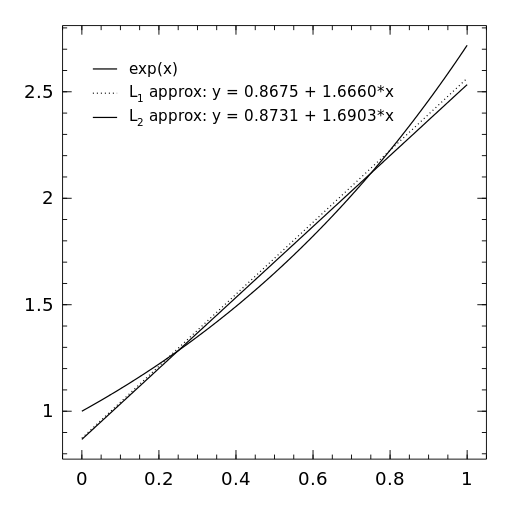
\includegraphics[height = 3in] {approx.png}


\p{4} Let $V$ be a finite dimensional inner product space and let $U$ be a subspace of $V$. Recall that the orthogonal complement of $U$ is 
$$U^\perp = \{v \in V | \langle v,u \rangle = 0 \text{ for all u } \in U\}.$$
Show that $V = U \oplus U^\perp$, where $\oplus$ symbolizes the direct sum of vector spaces. Also, show that $(U^\perp)^\perp = U$.
\begin{proof}
By HW 1 (4)(b), the orthogonal projection $P : V \to U$ exists.  Let $v \in V$. Then $v = Pv + (v - Pv)$. By HW 1 (3), $v - Pv \in U^\perp$. Hence, $V = U + U^\perp$.  Moreover, if $w \in U \cap U^\perp$, then $\langle w, w \rangle = 0$ so $w = 0$. Thus, $v = U \oplus U^\perp$.

To see that $U \subset (U^\perp)^\perp$, let  $u \in U$. Then $\langle v,u \rangle = 0$ for all $v \in U^\perp$. Hence, $\langle u,v \rangle = 0$ for all $v \in U^\perp$. Thus, $u \in (U^\perp)^\perp$.

Since $V = W \oplus W^\perp$ for any subspace $W$, we have $\dim (U) + \dim(U^\perp) = \dim (V) = \dim (U^\perp) + \dim((U^\perp)^\perp)$. Since $\dim(U^\perp) < \infty$, we have $\dim(U) = \dim((U^\perp)^\perp)$.  Since $U \subset (U^\perp)^\perp$ and they are finite dimensional, this implies that $U = (U^\perp)^\perp$.

\end{proof}


\end{document}
